\documentclass[tikz, border = 10pt]{standalone}


\usepackage{newpxtext,newpxmath}   % /upbeta
%\usepackage{fouriernc}            % /otherbeta
\usepackage{amsmath}
\renewcommand{\familydefault}{\sfdefault}
\usepackage{mathastext}

\usetikzlibrary{positioning, quotes, calc, math, arrows.meta, bending, shapes, backgrounds}

\tikzset{
every edge quotes/.style = {fill = white},
every node/.style = {scale = 1.1},
manifest/.style = {rectangle, draw, thin, inner sep = 3pt, minimum width = 1cm,
   minimum height = .85cm, align = center},
latent/.style = {ellipse, draw, thin, inner sep = 3pt, minimum width = 1cm,
   minimum height = .85cm},
residual1/.style = {circle, draw, thin, minimum size = 5mm, inner sep = 1pt},
residual2/.style = {rectangle, minimum width = 0.5pt, minimum height = 1.5mm,
   inner sep = 0pt, outer sep = 0mm},
regression/.style = {-{Stealth[length = 1.5mm]}, thin, shorten > = 1pt, 
   inner sep = 1.5pt, outer sep = 0mm},
covariance/.style={{Stealth[length = 1.5mm]}-{Stealth[length = 1.5mm]}, thin,
   shorten > = 1pt, shorten < = 1pt, inner sep = 1.5pt},
variance/.style={{Stealth[length = 1mm]}-{Stealth[length = 1mm]}, thin,
   shorten > = 1pt, shorten < = 1pt, inner sep = 1pt},
interaction/.style = {-{Stealth[sep = 1pt, length = 1.5mm] . Circle[length = 4pt]},
   thin, shorten > = -2pt},
constant/.style = {draw, thin, inner sep = 1pt, regular polygon,
   regular polygon sides = 3, minimum size = 5mm},
group/.style = {rectangle, inner sep = 2pt, minimum width = 15mm, minimum height = 5mm, 
   align = center}
}

\begin{document}
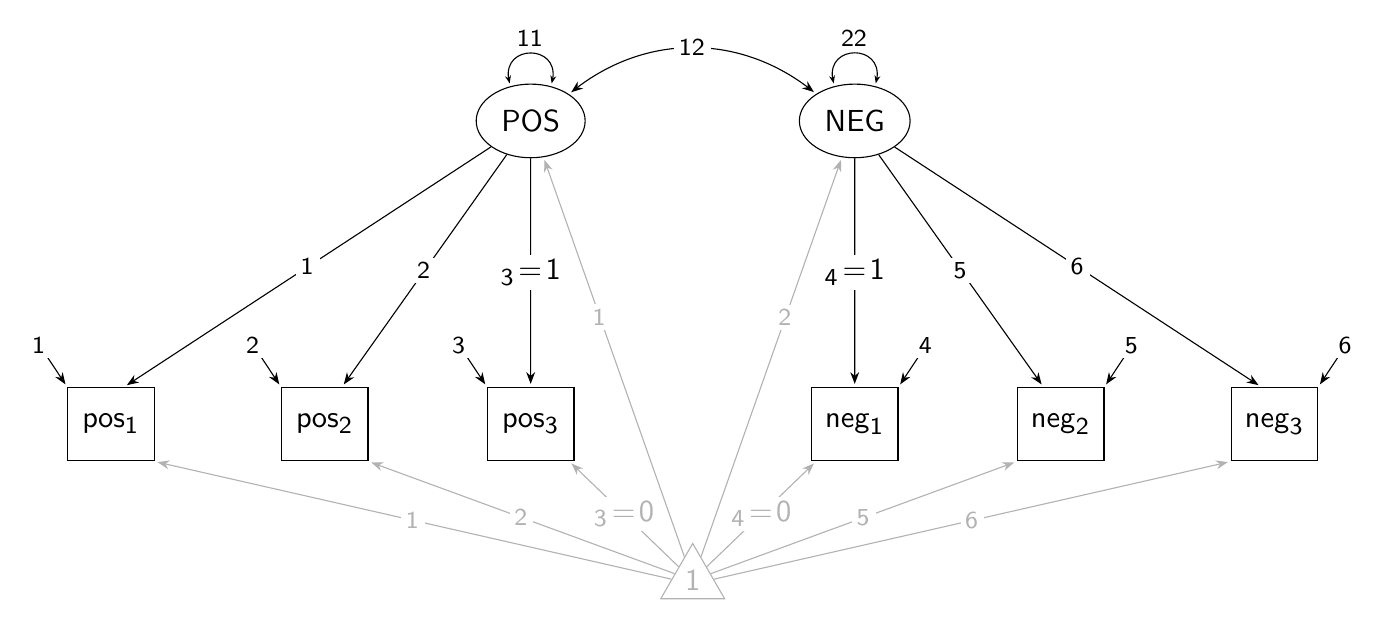
\begin{tikzpicture}

%% pos manifests
\node [manifest] (pos1) {$pos_1$};
\node [manifest] (pos2) [right = 1.6cm of pos1] {$pos_2$};
\node [manifest] (pos3) [right = 1.5cm of pos2] {$pos_3$};

%% neg manifests
\node [manifest] (neg1) [right = 3cm of pos3] {$neg_1$};
\node [manifest] (neg2) [right = 1.5cm of neg1] {$neg_2$};
\node [manifest] (neg3) [right = 1.6cm of neg2] {$neg_3$};

%% POS and NEG latents
\node [latent] (POS) [above = 2.9cm of pos3] {$POS$};
\node [latent] (NEG) [above = 2.9cm of neg1] {$NEG$};

%% Loadings
\path [regression] (POS) edge ["$\uplambda_1$"] (pos1.70);
\path [regression] (POS) edge ["$\uplambda_2$"] (pos2.65);
\path [regression] (POS) edge ["$\uplambda_3\!=\!1$"] (pos3.90);

\path [regression] (NEG) edge ["$\uplambda_4\!=\!1$"] (neg1.90);
\path [regression] (NEG) edge ["$\uplambda_5$"] (neg2.115);
\path [regression] (NEG) edge ["$\uplambda_6$"] (neg3.110);

%% Latent variances and covariance
\path [covariance] (POS.35) edge ["$\upphi_{12}$", bend left = 40] (NEG.145);
\path [variance] (POS.120) edge ["$\upphi_{11}$", above, outer sep = 1pt, bend left = 110, looseness = 3] (POS.60);
\path [variance] (NEG.120) edge ["$\upphi_{22}$", above, outer sep = 1pt, bend left = 110, looseness = 3] (NEG.60);

%% Residuals
\node [residual2] (e1) [above left = .65cm of pos1, xshift = 1mm] {};
\path [regression] (e1) edge ["$\uptheta_1$", pos = 0] (pos1.north west);

\node [residual2] (e2) [above left = .65cm of pos2, xshift = 1mm] {};
\path [regression] (e2) edge ["$\uptheta_2$", pos = 0] (pos2.north west);

\node [residual2] (e3) [above left = .65cm of pos3, xshift = 1mm] {};
\path [regression] (e3) edge ["$\uptheta_3$", pos = 0] (pos3.north west);

\node [residual2] (e4) [above right = .65cm of neg1, xshift = -1mm] {};
\path [regression] (e4) edge ["$\uptheta_4$", pos = 0] (neg1.north east);

\node [residual2] (e5) [above right = .65cm of neg2, xshift = -1mm] {};
\path [regression] (e5) edge ["$\uptheta_5$", pos = 0] (neg2.north east);

\node [residual2] (e6) [above right = .65cm of neg3, xshift = -1mm] {};
\path [regression] (e6) edge ["$\uptheta_6$", pos = 0] (neg3.north east);

%% latent means
\node [constant, black!30] (M) [below = 1.5cm of $(pos3)!0.5!(neg1)$] {1};
\path [regression, black!30] (M) edge ["$\upkappa_1$", pos = .6] (POS);
\path [regression, black!30] (M) edge ["$\upkappa_2$", pos = .6] (NEG);

%% Intercepts
\path [regression, black!30] (M.177) edge ["$\uptau_1$"] (pos1.south east);
\path [regression, black!30] (M) edge ["$\uptau_2$"] (pos2.south east);
\path [regression, black!30] (M) edge ["$\uptau_3\!=\!0$"] (pos3);

\path [regression, black!30] (M) edge ["$\uptau_4\!=\!0$"] (neg1);
\path [regression, black!30] (M) edge ["$\uptau_5$"] (neg2.south west);
\path [regression, black!30] (M.3) edge ["$\uptau_6$"] (neg3.south west);

\end{tikzpicture}
\end{document}

